The specified values are \(L=0.445\,\mathrm m\), \(b=0.037\,\mathrm m\), \(h=0.003\,\mathrm m\), \(E=200\,\mathrm{GPa}\), and \(\rho=7850\,\mathrm{kg/m^3}\). Taking bending about the axis associated with thickness \(h\), the section properties are
\[
A=bh=1.11\times10^{-4}\,\mathrm{m^2},\quad m=\rho A=0.871\,\mathrm{kg/m},\quad
I=\frac{bh^3}{12}=8.33\times10^{-11}\,\mathrm{m^4},
\]
\[
EI=16.7\,\mathrm{N\,m^2},\qquad a=(EI/m)^{1/4}=2.09\,\mathrm{m/\sqrt{s}}.
\]
For the first mode, $z_1=\pi$ and $\gamma_1=\pi/0.445=7.06\,\mathrm{rad/m}$. Substituting the section properties gives $\omega_1=\gamma_1^2\sqrt{EI/m}=217.9\,\mathrm{rad/s}$ and $f_1=\omega_1/(2\pi)=34.7\,\mathrm{Hz}$. Since $\gamma_j=j\gamma_1$, each frequency is $j^2$ times the first. Applying the roots and frequency equation from C.4 gives the following results. The coefficient \(\beta_j\) used for cantilever hyperbolic combinations is not needed here because both hyperbolic coefficients vanish.
\begin{center}
\begin{tabular}{rrrrr}
\toprule
\(j\)&\(z_j\)&\(\gamma_j\) (rad/m)&\(\omega_j\) (rad/s)&\(f_j\) (Hz)\\
\midrule
1&3.142&7.06&218&34.7\\
2&6.28&14.12&871&139\\
3&9.42&21.2&1961&312\\
4&12.57&28.2&3486&555\\
5&15.71&35.3&5447&867\\
\bottomrule
\end{tabular}
\end{center}
Figure~\ref{fig:hw03-c5-modes} shows \(W_j=\sin(j\pi x/L)\). Each curve has unit peak magnitude. For the unit-integral shapes \(\phi_j=\sqrt{2/L}W_j\), trapezoidal integration on 1000 equally spaced points produces the identity Gram matrix to floating-point precision. Frequency rises as \(j^2\), reflecting the fourth spatial derivative in the beam equation.
\begin{figure}[H]
\centering
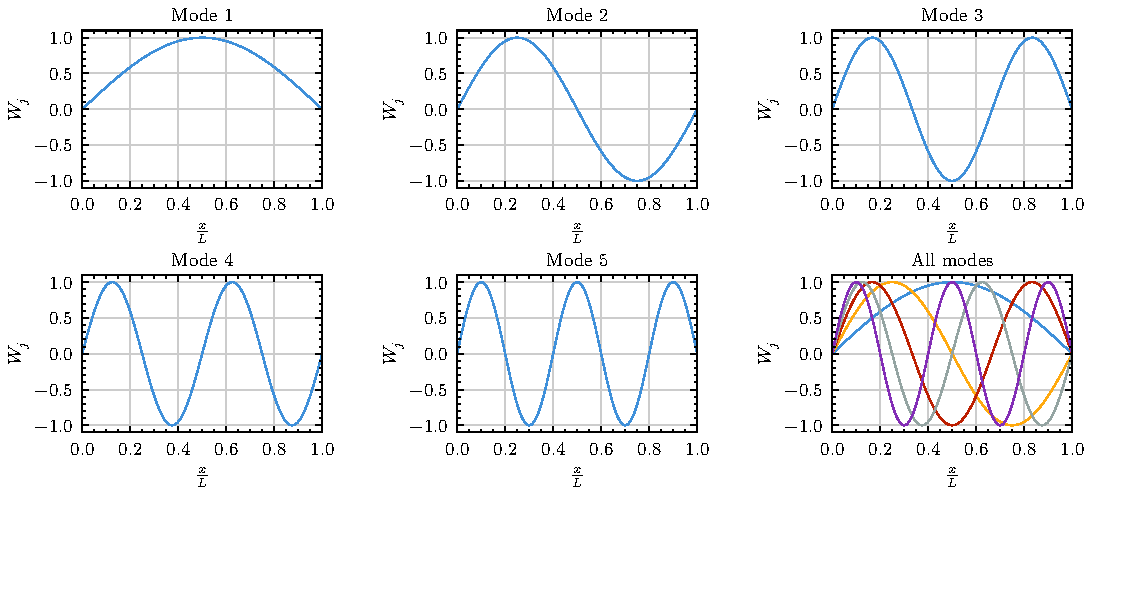
\includegraphics[width=\linewidth]{figures/generated/solutions/C5_modes.pdf}
\caption{Five simply supported beam modes and their overlay.}
\label{fig:hw03-c5-modes}
\end{figure}
The following script displays the inputs, results, and Gram matrix.
\lstinputlisting[style=hwmatlab]{matlab/C5.m}
